\section{Including Quadrupolar and Higher Order Interactions}
\label{qint}


The module {\prg Cfield} allows also to calculate systems with higher order interactions such
as quadrupolar interactions. Quadrupolar and higher order interactions can be calculated, which
can be described by products of Stevens operators. The general two ion exchange coupling is

\begin{equation}
\label{multipolehamiltonrepeated}
 {\mathcal H}_{JJ}=
             -\frac{1}{2}  \sum_{ss'} \sum_ {ll'} \sum_{mm'}
     {\mathcal K}_{ll'}^{mm'}(ss') O_{lm}({\mbf J}^s) O_{l'm'}({\mbf J}^s)
\end{equation}

For further information on the notation and symmetry restrictions to the
parameters in the Hamiltonian refer to~\cite{jensen91-1}~\footnote{\em http://www.nbi.ku.dk/page40667.htm}.


\subsection{Setting up {\prg mcphas.j\index{mcphas.j}} and other input files}

In order to include the higher order interactions, the number of columns in the input file
{\prg mcphas.j\index{mcphas.j}} has to be increased. The additional columns then contain the higher order
exchange constants.

Using the module {\prg Cfield}, the input file {\prg mcphas.j\index{mcphas.j}} may look as given for the 
example GdRu$_2$Si$_2$ in {\prg examples/gdru2si2}:

{\footnotesize
\begin{verbatim}
# GdRu2Si2 anisotropic bilinear and biquadratic exchange 
#<!--mcphase.mcphas.j-->
#***************************************************************
# Lattice and Exchange Parameter file for
# mcphas version 3.0
# - program to calculate static magnetic properties
# reference: M. Rotter JMMM 272-276 (2004) 481
# mcdisp version 3.0
# - program to calculate the dispersion of magnetic excitations
# reference: M. Rotter et al. J. Appl. Phys. A74 (2002) 5751
#***************************************************************
#
# Lattice Constants (A)
#! a=4.165 b=4.165 c=9.654 alpha=  90 beta=  90 gamma=  90
#! r1a= 0.5 r2a=   0 r3a=   0
#! r1b= 0.5 r2b=   1 r3b=   0   primitive lattice vectors [a][b][c]
#! r1c= 0.5 r2c=   0 r3c=   1
#! nofatoms=1  nofcomponents=8  number of atoms in primitive unit cell/number of components of each spin
#****************************************************************************}
#! da=   0 [a] db=   0 [b] dc=   0 [c] nofneighbours=38 diagonalexchange=1 gJ=   2 cffilename=Gd3p_cfield.sipf
# da[a]    db[b]      dc[c]       Jaa[meV]  Jbb[meV]  Jcc[meV]  Jab[meV]  Jba[meV]  Jac[meV]  Jca[meV]  Jbc[meV]  %%@
Jcb[meV]} 
-1.0 0.0 0.0 0.08390 0.08390 0.21890 -0.0024 -0.0096 -0.0008 -0.0096 -0.0024 
1.0 0.0 0.0 0.08390 0.08390 0.21890 -0.0024 -0.0096 -0.0008 -0.0096 -0.0024 
0.0 -1.0 0.0 0.08390 0.08390 0.21890 -0.0024 -0.0096 -0.0008 -0.0096 -0.0024 
0.0 1.0 0.0 0.08390 0.08390 0.21890 -0.0024 -0.0096 -0.0008 -0.0096 -0.0024 
-0.5 -0.5 -0.5 0.00380 0.00380 0.01000 0.0 0.0 0.0 0.0 0.0 
-0.5 -0.5 0.5 0.00380 0.00380 0.01000 0.0 0.0 0.0 0.0 0.0 
-0.5 0.5 -0.5 0.00380 0.00380 0.01000 0.0 0.0 0.0 0.0 0.0 
-0.5 0.5 0.5 0.00380 0.00380 0.01000 0.0 0.0 0.0 0.0 0.0 
0.5 -0.5 -0.5 0.00380 0.00380 0.01000 0.0 0.0 0.0 0.0 0.0 
0.5 -0.5 0.5 0.00380 0.00380 0.01000 0.0 0.0 0.0 0.0 0.0 
0.5 0.5 -0.5 0.00380 0.00380 0.01000 0.0 0.0 0.0 0.0 0.0 
0.5 0.5 0.5 0.00380 0.00380 0.01000 0.0 0.0 0.0 0.0 0.0 
-1.0 -1.0 0.0 -0.03630 -0.03630 -0.09445 0.0 0.0 0.0 0.0 0.0 
-1.0 1.0 0.0 -0.03630 -0.03630 -0.09445 0.0 0.0 0.0 0.0 0.0 
1.0 -1.0 0.0 -0.03630 -0.03630 -0.09445 0.0 0.0 0.0 0.0 0.0 
1.0 1.0 0.0 -0.03630 -0.03630 -0.09445 0.0 0.0 0.0 0.0 0.0 
1.5 -0.5 0.5 -0.00072 -0.00072 -0.00188 0.0 0.0 0.0 0.0 0.0 
-1.5 -0.5 0.5 -0.00072 -0.00072 -0.00188 0.0 0.0 0.0 0.0 0.0 
1.5 -0.5 -0.5 -0.00072 -0.00072 -0.00188 0.0 0.0 0.0 0.0 0.0 
0.5 -1.5 0.5 -0.00072 -0.00072 -0.00188 0.0 0.0 0.0 0.0 0.0 
0.5 1.5 0.5 -0.00072 -0.00072 -0.00188 0.0 0.0 0.0 0.0 0.0 
0.5 1.5 -0.5 -0.00072 -0.00072 -0.00188 0.0 0.0 0.0 0.0 0.0 
-0.5 1.5 0.5 -0.00072 -0.00072 -0.00188 0.0 0.0 0.0 0.0 0.0 
-1.5 -0.5 -0.5 -0.00072 -0.00072 -0.00188 0.0 0.0 0.0 0.0 0.0 
1.5 0.5 0.5 -0.00072 -0.00072 -0.00188 0.0 0.0 0.0 0.0 0.0 
-1.5 0.5 -0.5 -0.00072 -0.00072 -0.00188 0.0 0.0 0.0 0.0 0.0 
-0.5 -1.5 -0.5 -0.00072 -0.00072 -0.00188 0.0 0.0 0.0 0.0 0.0 
-0.5 -1.5 0.5 -0.00072 -0.00072 -0.00188 0.0 0.0 0.0 0.0 0.0 
1.5 0.5 -0.5 -0.00072 -0.00072 -0.00188 0.0 0.0 0.0 0.0 0.0 
-0.5 1.5 -0.5 -0.00072 -0.00072 -0.00188 0.0 0.0 0.0 0.0 0.0 
-1.5 0.5 0.5 -0.00072 -0.00072 -0.00188 0.0 0.0 0.0 0.0 0.0 
0.5 -1.5 -0.5 -0.00072 -0.00072 -0.00188 0.0 0.0 0.0 0.0 0.0 
-2.0 0.0 0.0 -0.01754 -0.01754 -0.04567 0.0 0.0 0.0 0.0 0.0 
2.0 0.0 0.0 -0.01754 -0.01754 -0.04567 0.0 0.0 0.0 0.0 0.0 
0.0 -2.0 0.0 -0.01754 -0.01754 -0.04567 0.0 0.0 0.0 0.0 0.0 
0.0 2.0 0.0 -0.01754 -0.01754 -0.04567 0.0 0.0 0.0 0.0 0.0 
0.0 0.0 1.0 0.24850 0.24850 0.13560 0.0 0.0 0.0 0.0 0.0 
0.0 0.0 -1.0 0.24850 0.24850 0.13560 0.0 0.0 0.0 0.0 0.0 
\end{verbatim}
}
here the meaning of the Jaa, Jbb, Jcc, Jdd, Jee \dots is the exchange ${\mathcal K}_{ll'}^{mm'}(ss')$ between %%@
$O_1^1(s)$, $O_1^0(c)$,$O_1^1(c)$, $O_2^2(s)$, $O_2^1(s)$,$O_2^0(c)$,$O_2^1(c)$,$O_2^2(c)$,$O_3^3(s)$, ...
according to equation table~\ref{olms}.
 The exchange constants for the
products of these Stevens operators have to be 
given according to the following scheme:

\begin{verbatim}
   aa bb cc ab ba ac ca bc cb (3x3 matrix)
   aa bb cc dd ab ba ac ca ad da bc cb bd db cd dc (4x4 matrix)
   aa bb cc dd ee ab ba ac ca ad da ae ea bc cb bd db be eb cd dc ce ec de ed (5x5 matrix)
   etc ...
\end{verbatim}

The other input and output files have the same format as usual, but with the modification, that
there are now $n$ components of the 'spins' instead of 3 ($<J_a>$,$<J_b>$,$<J_c>$).
The components $<J_a>$,$<J_b>$,$<J_c>$,$<J_d>$,$<J_e>$, etc. correspond to $<O_{11}(s)>$, $<O_{10}>$,
$<O_{11}>$, $<O_{22}(s)>$, $<O_{21}(s)>$,$<O_{20}>$,$<O_{21}>$,$<O_{22}>$,$<O_{33}(s)>$, ...
 respectively. Table~\ref{olms} contains a list of first and second order Stevens parameters.
For a full list please refer to appendix~\ref{stevens}.

\begin{table}[hb] 
\begin{center}  
\caption {Stevens operator equivalents $O_l^m$ and corresponding notation used in module {\prg %%@
cfield\index{cfield}} 
($J_{\pm}=J_x\pm iJ_y=J_c\pm iJ_a$ ). For a full list please refer to appendix~\ref{stevens}.}   
\label{olms}   
\begin{tabular} 
{lr} 
Stevens Operator & Notation used in module {\prg cfield\index{cfield}} \\
\hline
$O_{00}=1$ ($O_0^0(s)=0$) &\\
\hline
$O_{11}(s)=\frac{-i}{2}[J_+-J_-]=J_y$ &  $J_a$\\
$O_{10}=J_z$  ($O_1^0(s)=0$) & $J_b$ \\
$O_{11}=\frac{1}{2}[J_++J_-]=J_x$ &  $J_c$\\
\hline
$O_{22}(s)=\frac{-i}{2}[J_+^2-J_-^2]=J_xJ_y+J_yJ_x$($=2P_{xy}$) & $J_d$ \\
$O_{21}(s)=\frac{-i}{4}[(J_+-J_-)J_z+J_z(J_+-J_-)]=\frac{1}{2}[J_yJ_z+J_zJ_y]$($=P_{yz}$) & $J_e$ \\
$O_{20}=[3J_z^2-J(J+1)]$ ($O_2^0(s)=0$) & $J_f$ \\
$O_{21}=\frac{1}{4}[(J_++J_-)J_z+J_z(J_++J_-)]=\frac{1}{2}[J_xJ_z+J_zJ_x]$($=P_{xz}$) & $J_g$ \\
$O_{22}=\frac{1}{2}[J_+^2+J_-^2]=[J_x^2-J_y^2]$ & $J_h$ \\
\hline
 \end{tabular}
\end{center}   
\end{table}

The {\prg indexexchange} parameter discussed in section~\ref{mcphasj} may be useful in keeping the input
of the exchange components short. For example the $\zeta$ and $\eta$ strain modes on the quasi-cubic sites
of a double hexagonal close packed structure involves the coupling of $P_{zx}$ ($J_g$) and $P_{xy}$ ($J_d$) 
as well as $P_{yz}$ ($J_e$) and $O_2^2$ $(J_h)$ quadrupoles, so the {\prg diagonalexchange=1} option 
cannot be used. Thus 64 components need to be specified to describe the $8\times 8$ exchange tensor. 
However, we can simplify this with the {\prg indexexchange} parameter by setting {\prg diagonalexchange=2}, 
as follows for UPd$_3$:

{\footnotesize \begin{verbatim}
# UPd3 
#<!--mcphase.mcphas.j-->
#! a=9.92465 b=5.73 c=9.65  alpha=  90 beta=  90 gamma=  90
#! r1x= 1 r2x=   0 r3x=   0
#! r1y= 0 r2y=   1 r3y=   0
#! r1z= 0 r2z=   0 r3z=   1
#! nofatoms=1 nofcomponents=8
#*************************************************************************
#! x=   0 [a] y=   0 [b] z=   0 nofneighbours=6 diagonalexchange=2 gJ=0.8 cffilename=mcphas.cf1
#! x[a]  y[b]    z[c]   Ja[meV]  Jb[meV]  Jc[meV]  Jd[meV]  Je[meV]  Jf[meV]  Jg[meV]  Jh[meV]
#! symmetricexchange=1 indexexchange= JaJa JbJb JcJc JdJd JeJe JfJf JgJg JhJh JgJd JhJe
 0    0    0.5 -0.022 -0.022 -0.022  0.0035198 -0.18643  -0.00053332 -0.18643   0.00087996  0.013      0.0064378
 0    0   -0.5 -0.022 -0.022 -0.022  0.0035198 -0.18643  -0.00053332 -0.18643   0.00087996  0.013      0.0064378
 0.5  0.5  0   -0.022 -0.022 -0.022 -0.0034195 -0.019714 -0.00034044 -0.019714 -0.00085486 -0.0065221 -0.0050197
-0.5 -0.5  0   -0.022 -0.022 -0.022 -0.0034195 -0.019714 -0.00034044 -0.019714 -0.00085486 -0.0065221 -0.0050197
 0.5 -0.5  0   -0.022 -0.022 -0.022 -0.0034195 -0.019714 -0.00034044 -0.019714 -0.00085486 -0.0065221 -0.0050197
-0.5  0.5  0   -0.022 -0.022 -0.022 -0.0034195 -0.019714 -0.00034044 -0.019714 -0.00085486 -0.0065221 -0.0050197
\end{verbatim} }

\subsection{Running {\prg McPhase} and {\prg McDisp}}

The programs {\prg mcphas} and {\prg mcdisp\index{mcdisp}} are run completely the same way as usual, only
the output files contain also information about the (thermal) expectation values of $<O_l^m>$
dependent on temperature and magnetic field. 
Using the module cfield the notation $<J_a>$,$<J_b>$,$<J_c>$,
$<J_d>$, $<J_e>$, etc. correspond to $<O_{11}(s)>$, $<O_{10}>$,
$<O_{11}>$, $<O_{22}(s)>$, $<O_{21}(s)>$,$<O_{20}>$,$<O_{21}>$,$<O_{22}>$,$<O_{33}(s)>$, ...
 respectively.
Note that by the higher order interactions not only the static properties are changed, but also the
dispersion of the magnetic excitations is influenced.


The directory {\prg examples/gdru2si2} contains an example of a simulation of biquadratic (i.e. isotropic %%@
quadrupolar) interactions leading to an improved description of magnetic susceptibility.

For DyCu$_2$ the conversion
of the magnetic axis due to quadrupolar exchange has been calculated according to the model 
\cite{yoshida98-1421}. The calculated quadrupolar phase diagram is shown in figure~\ref{qphased}.

\begin{figure}[hb]%h=here, t=top, b=bottom, p=separate figure page
\begin{center}\leavevmode
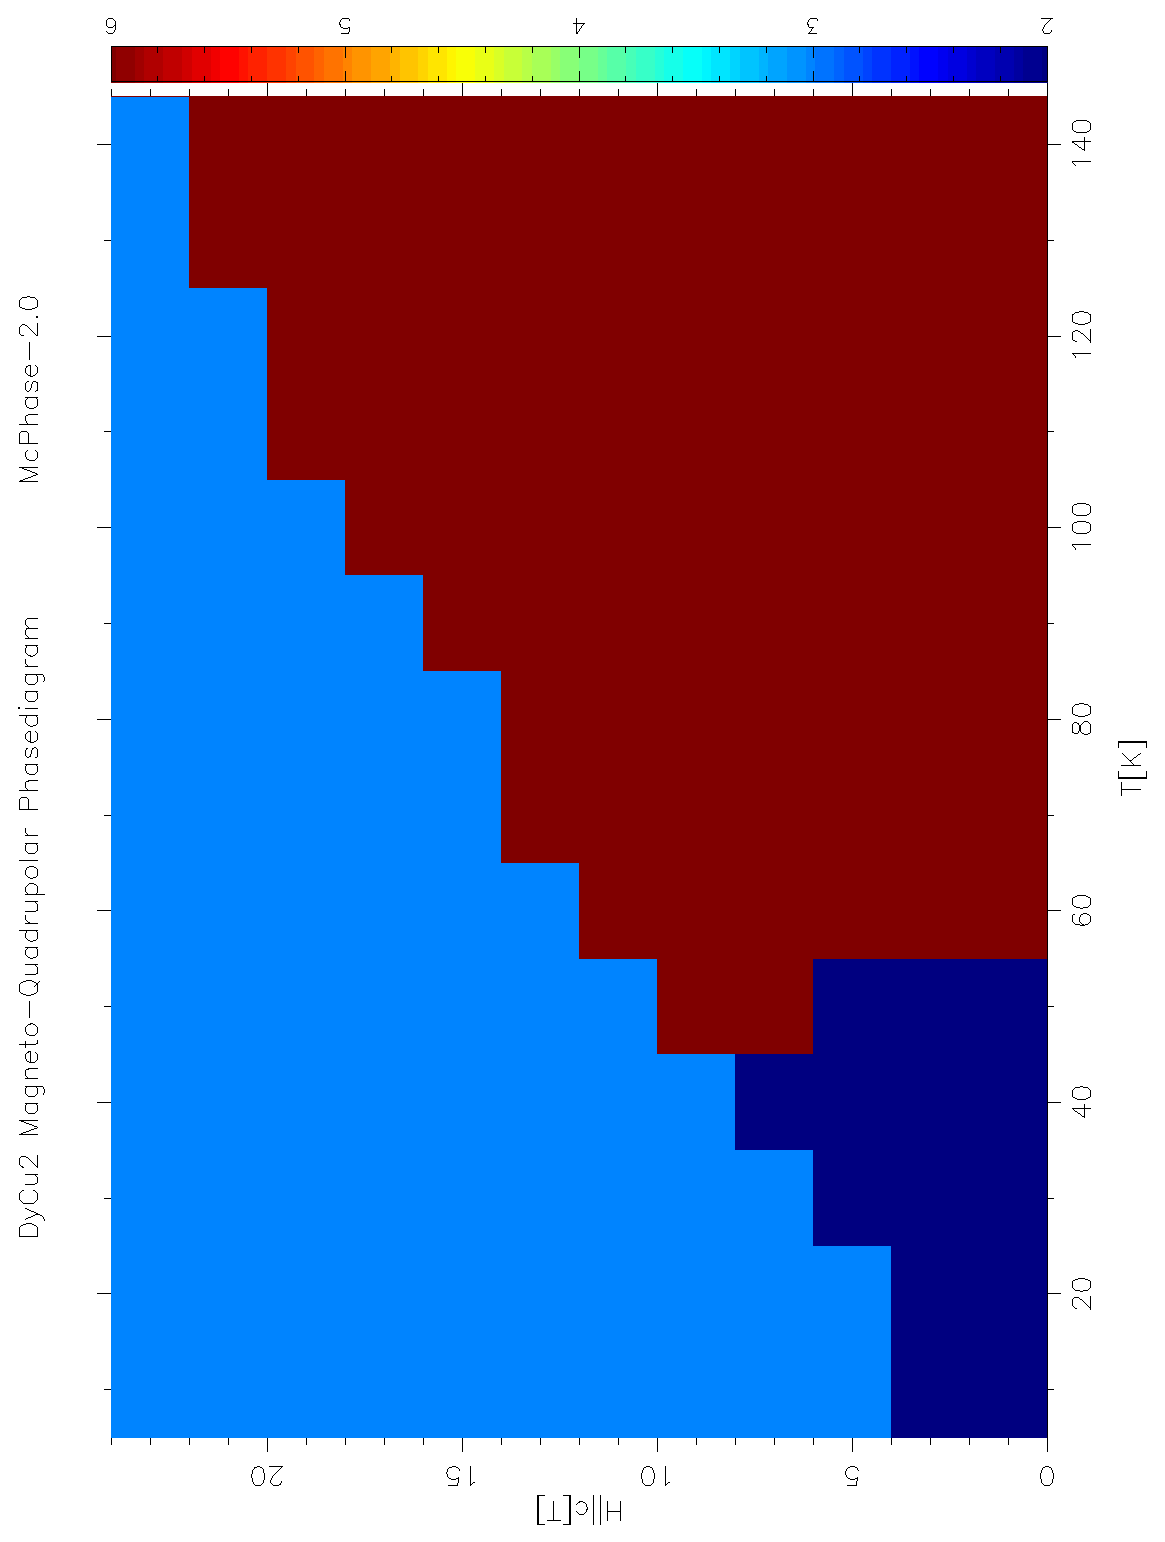
\includegraphics[angle=-90, width=0.5\textwidth]{./figsrc/dyphased.ps}
\end{center}
\caption{DyCu$_2$: calculated quadrupolar phased diagram. When applying a large magnetic field
parallel to the $c$ axis of the orthorhombic crystal, the system undergoes a structural transformation
associated with a reorientation of the structural unit cell. This effect can be modelled by a large
quadrupolar interaction.[plot created with program {\prg phased}]}
\label{qphased}
\end{figure}

When large  quadrupolar interactions are present, the excitation spectrum is changed and
quadrupolar modes (orbitons) with a finite dispersion are expected. 
These modes correspond to an cooperative oscillation of the quadrupolar moments such as shown
in figure~\ref{qmodes}.
The program {\prg mcdisp\index{mcdisp}}
is able to calculate this dispersion and the corresponding neutron scattering cross section as shown
in figure~\ref{qintensity} for the case of PrCu$_2$. 
 

\begin{figure}[hb]%h=here, t=top, b=bottom, p=separate figure page
\begin{center}\leavevmode
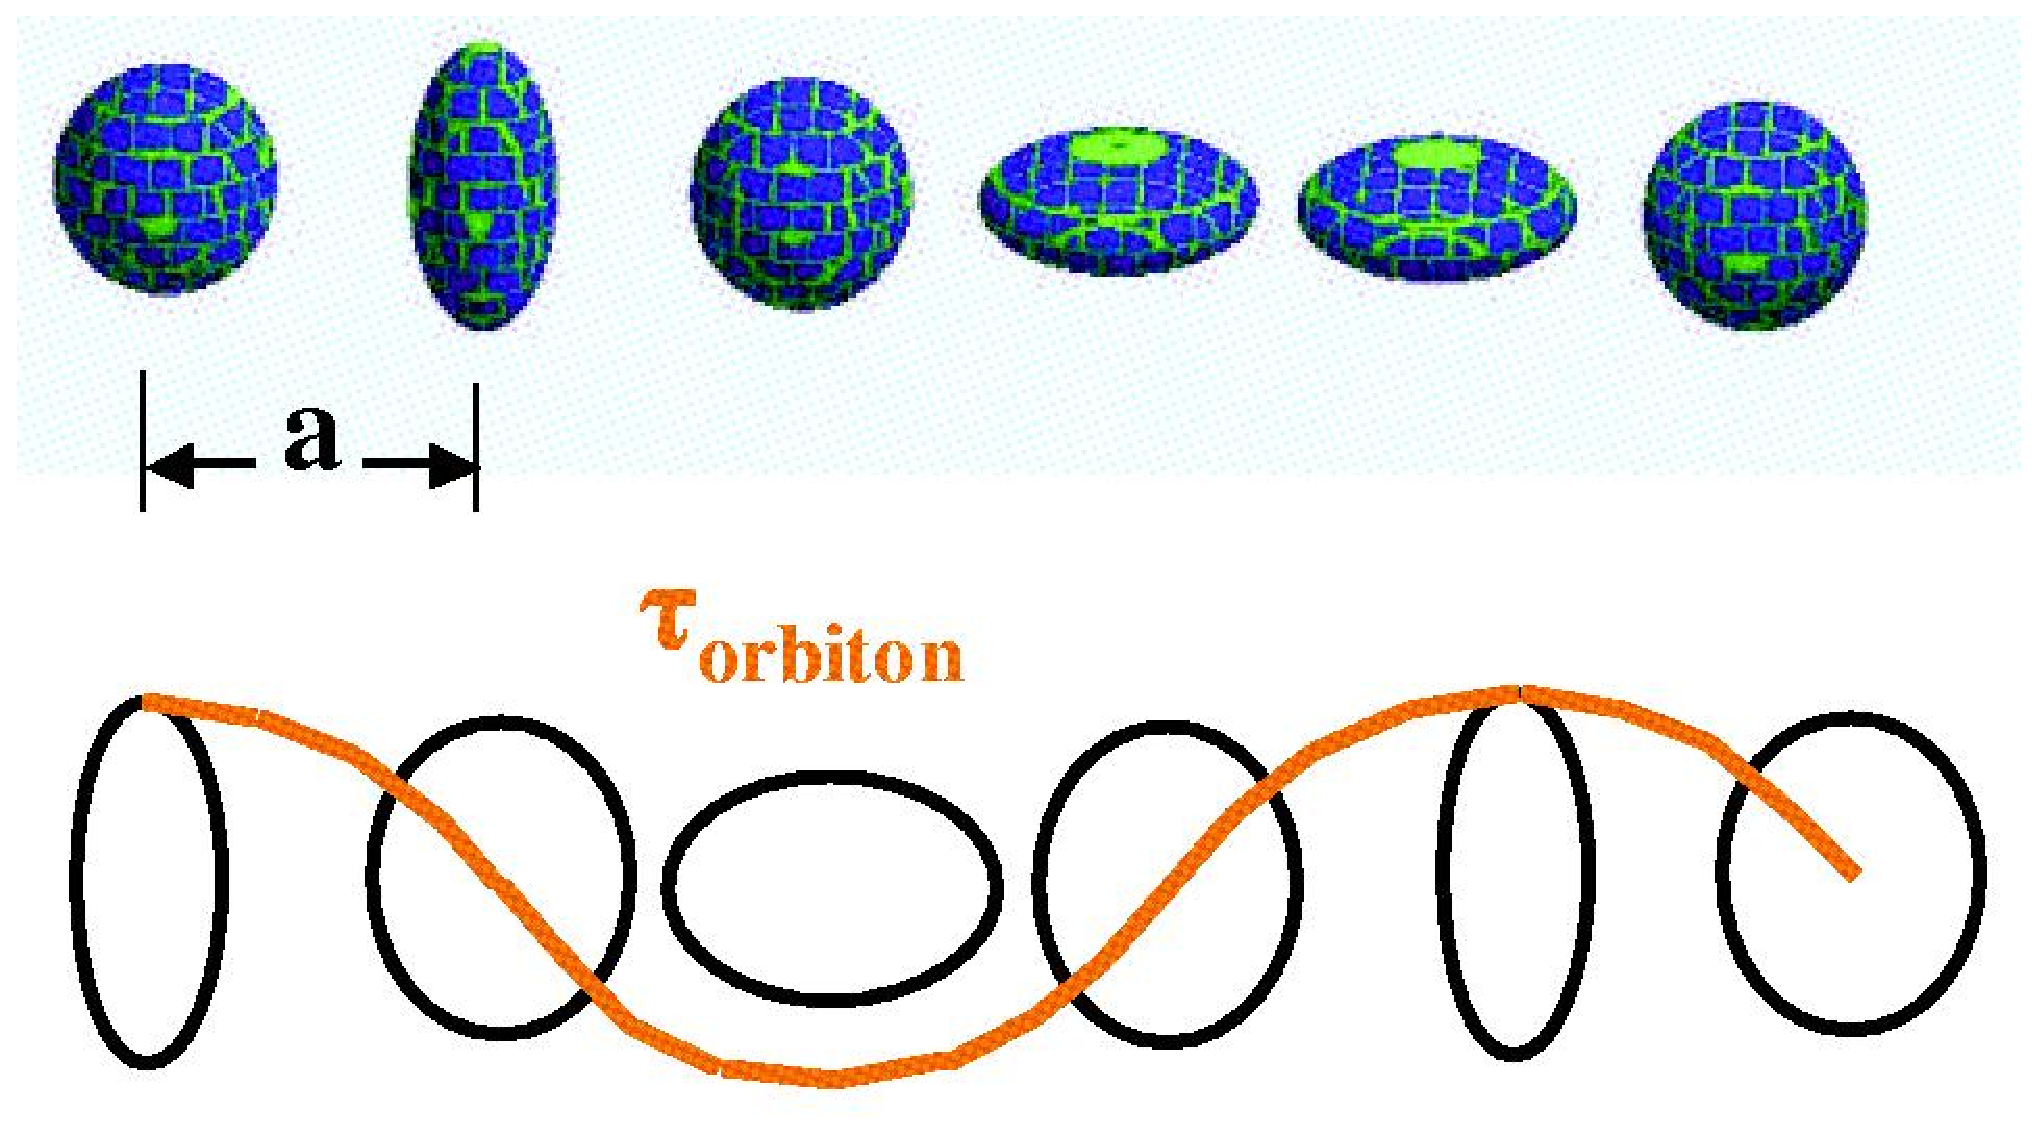
\includegraphics[angle=0, width=0.6\textwidth]{./figsrc/orbiton.ps}
\end{center}
\caption{Orbital excitations viewed  as correlated changes in 4f-charge densities.}
\label{qmodes}
\end{figure}

\begin{figure}[hb]%h=here, t=top, b=bottom, p=separate figure page
\begin{center}\leavevmode
\includegraphics[angle=0, width=0.5\textwidth]{./figsrc/prcu2_0k0_5T.eps}
\end{center}
\caption{PrCu$_2$: calculated dispersion of quadrupolar excitations in a field of 5 Tesla parallel to the $a$ axis %%@
of this orthorhombic system.
[plot created with program {\prg displaycontour\index{displaycontour}}]}
\label{qintensity}
\end{figure}
